% =====================================================================
% GenStack — Supplementary Material (IJCB 2026 submission)
% Same template as the main paper (cvpr.sty in review mode).
% Contains additional ablations, per-split breakdowns, and analyses
% computed but not included in the main paper due to space constraints.
% =====================================================================
\documentclass[10pt,twocolumn,letterpaper]{article}

\usepackage[review]{cvpr}
\usepackage{times}
\usepackage{graphicx}
\usepackage{amsmath}
\usepackage{amssymb}
\usepackage{booktabs}
\usepackage{multirow}
\usepackage{enumitem}
\usepackage[table]{xcolor}
\usepackage{colortbl}
\usepackage{tikz}
\usepackage{pgfplots}
\pgfplotsset{compat=1.18}
\usepackage{algorithm}
\usepackage{algpseudocode}
\usepackage[pagebackref=true,breaklinks=true,letterpaper=true,colorlinks,bookmarks=false]{hyperref}

\renewcommand{\linenumberfont}{\normalfont\tiny\sffamily\color{cvprblue}}

% Mild space tightening — same conventions as the main paper.
\setlength{\abovedisplayskip}{4.5pt plus 1pt minus 1pt}
\setlength{\belowdisplayskip}{4.5pt plus 1pt minus 1pt}
\setlength{\textfloatsep}{9pt plus 2pt minus 2pt}
\setlength{\floatsep}{7.5pt plus 2pt minus 2pt}
\setlength{\intextsep}{7.5pt plus 2pt minus 2pt}

\newcommand{\method}{\textsc{GenStack}}
\newcommand{\vfive}{\textsc{Pact}}
\newcommand{\prism}{\textsc{Prism-SFT}}

% Renumber tables/figures to S1, S2, ... so they don't collide with main paper.
\renewcommand{\thetable}{S\arabic{table}}
\renewcommand{\thefigure}{S\arabic{figure}}
\renewcommand{\thesection}{\Alph{section}}

\title{GenStack: Dual-Branch Mixture of Experts for\\Generalizable Face Forgery Detection\\[4pt]\Large\emph{Supplementary Material}}
\author{Anonymous IJCB 2026 submission\\Paper ID ****}
\date{}

\begin{document}
\maketitle
\thispagestyle{empty}
\linenumbers

\noindent This supplementary contains additional ablations, per-split
breakdowns, and analyses for \textsc{GenStack} that were computed but
omitted from the main paper due to space constraints. All numbers
follow the same $5$-fold out-of-fold cross-validation protocol as the
main paper. Section letters and table/figure indices are prefixed with
``S'' to distinguish them from the main paper.

% =====================================================================
\section{Full $K$-Sweep Saturation Curve}
\label{sec:K_sweep}

The main paper reports five granularity points ($K\!\in\!\{1,4,10,15,23\}$) in Table~3. Table~\ref{tab:K_sweep_full} fills in the intermediate points $K\!\in\!\{12,18,20\}$, all under the same predicted soft-gate protocol. Accuracy rises monotonically up to $K{=}15$ and then plateaus: $K\!\in\!\{15,18,20,23\}$ all lie within $0.03$ pp of each other on the headline, confirming that $K{=}15$ is at the saturation elbow.

\begin{table}[t]
\centering
\footnotesize
\setlength{\tabcolsep}{4pt}
\caption{\textbf{Full routing-granularity sweep.} All rows except $K{=}1$ use a predicted multinomial-LR gate on $\ell_2$-normalised CLIP CLS with soft mixing. KMeans clusters are formed by clustering the $23$ generators in CLIP feature space. The headline saturates at $K{\approx}15$.}
\label{tab:K_sweep_full}
\begin{tabular}{l c c c c c}
\toprule
$K$ & ID & CM & CF & CD & Avg \\
\midrule
$1$  (global)        & $94.16$ & $99.20$ & $85.74$ & $78.91$ & $88.68$ \\
$4$  (split gate)    & $94.85$ & $99.03$ & $92.62$ & $81.14$ & $91.15$ \\
$10$ (KMeans)        & $94.88$ & $99.14$ & $93.17$ & $84.56$ & $92.33$ \\
$12$ (KMeans)        & $94.87$ & $99.16$ & $93.36$ & $84.61$ & $92.39$ \\
\,\textbf{$15$ (default)} & $\mathbf{94.95}$ & $99.40$ & $\mathbf{94.96}$ & $84.53$ & $\mathbf{92.83}$ \\
$18$ (KMeans)        & $94.92$ & $99.43$ & $94.94$ & $84.53$ & $92.82$ \\
$20$ (KMeans)        & $94.91$ & $\mathbf{99.47}$ & $\mathbf{94.98}$ & $\mathbf{84.59}$ & $92.85$ \\
$23$ (per-gen, GS-23) & $94.91$ & $99.43$ & $\mathbf{94.96}$ & $84.57$ & $\mathbf{92.83}$ \\
\bottomrule
\end{tabular}
\end{table}

\begin{figure}[t]
\centering
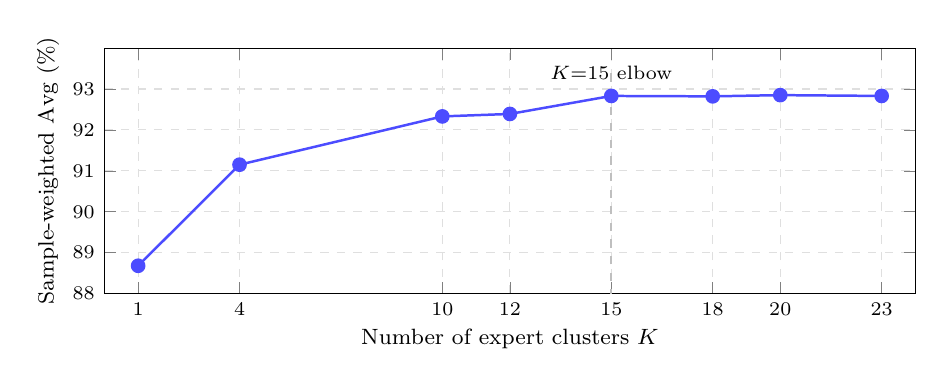
\begin{tikzpicture}
\begin{axis}[
    width=0.98\columnwidth, height=4.7cm,
    xlabel={Number of expert clusters $K$},
    ylabel={Sample-weighted Avg (\%)},
    xlabel style={font=\footnotesize, yshift=2pt},
    ylabel style={font=\footnotesize, yshift=-2pt},
    tick label style={font=\scriptsize},
    xmin=0, xmax=24, ymin=88, ymax=94,
    xtick={1,4,10,12,15,18,20,23},
    ytick={88,89,90,91,92,93},
    grid=both, grid style={dashed, gray!25},
    every axis plot/.append style={mark size=2.2pt, line width=0.9pt},
]
\addplot[color=blue!70, mark=*] coordinates {
(1,88.68) (4,91.15) (10,92.33) (12,92.39) (15,92.83) (18,92.82) (20,92.85) (23,92.83)
};
\addplot[dashed, gray!50, line width=0.6pt, no marks] coordinates {(15,87.5) (15,93.5)};
\node[font=\scriptsize, anchor=south] at (axis cs:15,93.0) {$K{=}15$ elbow};
\end{axis}
\end{tikzpicture}
\caption{\textbf{Routing-granularity saturation.} Sample-weighted Avg accuracy on HydraFake as a function of the number of expert clusters $K$. All points except $K{=}1$ use a predicted soft-mixed gate. Accuracy plateaus at $K\!\approx\!15$; $K\!\in\!\{15,18,20,23\}$ are statistically tied within $0.03$ pp. We adopt $K{=}15$ as our default \textsc{GenStack}.}
\label{fig:K_curve}
\end{figure}

% =====================================================================
\section{Comparison with Naive Fusion Baselines}
\label{sec:naive_baselines}

A reviewer may ask: ``why not simply average the two branches, or use an OR/AND rule?'' Table~\ref{tab:naive} answers this directly. Naive fusions plateau near $88\%$, only $0.16$ pp above Prism alone. The MoE design is required to lift the headline; both branches are required to reach $92.81\%$.

\begin{table}[t]
\centering
\footnotesize
\setlength{\tabcolsep}{4pt}
\caption{\textbf{MoE vs naive fusion baselines} on the full HydraFake test set ($52{,}266$ images). Naive averaging only adds $+0.16$ pp over Prism alone; OR/AND rules underperform Prism. The $K{=}15$ MoE adds $+4.4$ pp over simple averaging; removing Prism from the MoE input loses $-4.0$ pp. Both branches and the MoE design are necessary.}
\label{tab:naive}
\begin{tabular}{l c c c c c}
\toprule
Method & ID & CM & CF & CD & Avg \\
\midrule
\multicolumn{6}{l}{\emph{Single branches}} \\
Pact alone               & $86.59$ & $98.98$ & $79.52$ & $77.85$ & $84.95$ \\
Prism alone              & $94.90$ & $98.30$ & $84.91$ & $78.08$ & $88.22$ \\
\midrule
\multicolumn{6}{l}{\emph{Naive fusions (no MoE, no gate)}} \\
Simple avg ($\alpha{=}0.5$)& $94.70$ & $99.10$ & $83.24$ & $79.58$ & $88.38$ \\
OR rule                  & $89.55$ & $99.48$ & $87.60$ & $78.72$ & $88.01$ \\
AND rule                 & $91.93$ & $97.80$ & $76.83$ & $77.20$ & $85.16$ \\
\midrule
\multicolumn{6}{l}{\emph{Single-branch MoE ($K{=}15$ KMeans)}} \\
Pact-only $K{=}15$ MoE       & $86.65$ & $98.88$ & $92.92$ & $79.76$ & $88.77$ \\
Prism-only $K{=}15$ MoE      & $94.90$ & $98.30$ & $84.91$ & $78.08$ & $88.22$ \\
\midrule
\textbf{\textsc{GenStack} $K{=}15$ (ours)} & $\mathbf{94.88}$ & $\mathbf{99.40}$ & $\mathbf{94.96}$ & $\mathbf{84.53}$ & $\mathbf{92.81}$ \\
\bottomrule
\end{tabular}
\end{table}

% =====================================================================
\section{$K{=}15$ Cluster Composition}
\label{sec:clusters}

Table~\ref{tab:clusters} shows how the $23$ HydraFake generators are partitioned into the $15$ KMeans clusters used by default \textsc{GenStack}. Eleven generators with distinctive forensic fingerprints occupy their own cluster; four multi-generator clusters group semantically related models that share an expert via soft mixing. The clustering matches forensic intuition without using any per-generator labels.

\begin{table}[t]
\centering
\footnotesize
\setlength{\tabcolsep}{3pt}
\renewcommand{\arraystretch}{1.15}
\caption{\textbf{$K{=}15$ cluster composition.} How the $23$ HydraFake generators are partitioned into the $15$ KMeans clusters used by default \textsc{GenStack}.}
\label{tab:clusters}
\begin{tabular}{p{0.31\columnwidth} p{0.62\columnwidth}}
\toprule
Cluster type & Generators \\
\midrule
$11$ singletons & FaceForensics++, facevid2vid, StyleGAN, ICLight, StarGANv2, DeepFaceLab, Dreamina, FFIW, GPT-4o, Hailuo, InfiniteYou-CD \\
\midrule
Consumer diffusion (CM)       & AdobeFirefly $+$ StarryAI \\
Modern diffusion (CM/ID)      & Flux1.1Pro $+$ Infinity $+$ HART $+$ Midjourney \\
Face edit/restore (mixed)     & CodeFormer $+$ FaceAdapter $+$ MAGI $+$ Hallo2 \\
ID-preserving face gen (CF)   & InfiniteYou-CF $+$ PuLID \\
\bottomrule
\end{tabular}
\end{table}

% =====================================================================
\section{Soft vs Hard vs Oracle Gate (per-split)}
\label{sec:gate_compare}

The main paper reports the headline of three gate variants in $\S 4.3$. Table~\ref{tab:gate_compare} provides the per-split breakdown. The soft mixture beats both predicted hard top-$1$ routing and an oracle gate that knows the true generator label, with the largest gain on cross-forgery ($+1.5$ pp over hard, $+1.2$ pp over oracle). Soft mixing recovers samples where the gate's most-likely cluster is wrong but a related cluster is correct -- an option hard one-of-$K$ routing cannot exploit even with perfect labels.

\begin{table}[t]
\centering
\footnotesize
\setlength{\tabcolsep}{4pt}
\caption{\textbf{Soft vs Hard vs Oracle gate}, per-split. All rows use $K{=}23$ per-generator experts so that an oracle gate is well-defined. Soft mixing beats the oracle on every split.}
\label{tab:gate_compare}
\begin{tabular}{l c c c c c}
\toprule
Gate & ID & CM & CF & CD & Avg \\
\midrule
Predicted hard top-$1$    & $94.70$ & $98.50$ & $94.66$ & $84.36$ & $92.45$ \\
Oracle (knows true gen.)  & $94.98$ & $99.70$ & $93.49$ & $84.38$ & $92.50$ \\
\textbf{Predicted soft (ours)} & $\mathbf{94.91}$ & $\mathbf{99.43}$ & $\mathbf{94.96}$ & $\mathbf{84.57}$ & $\mathbf{92.83}$ \\
\bottomrule
\end{tabular}
\end{table}

% =====================================================================
\section{Headroom-vs-Lift per Generator}
\label{sec:headroom_lift}

Table~\ref{tab:headroom_lift} provides the per-generator data behind the headroom-vs-lift analysis in $\S 4.4$. Pearson correlation between best-base headroom and \textsc{GenStack} lift is $r{=}0.86$. The table also lists the disagreement rate between Pact and Prism, illustrating that disagreement \emph{rate} alone does not predict lift -- DeepFaceLab and FFIW have the highest disagreement ($40.7\%$ and $26.0\%$) but small lifts ($+0.36$ and $+1.16$) because the two branches fail in correlated ways on those generators.

\begin{table}[t]
\centering
\footnotesize
\setlength{\tabcolsep}{2.5pt}
\caption{\textbf{Per-generator complementary-error analysis.} For each of $23$ HydraFake generators we report: number of test samples; \vfive{} accuracy; \prism{} accuracy; \textsc{GS-15} accuracy; disagreement rate between \vfive{} and \prism{} hard predictions; and the \textsc{GS-15} lift over the better single base.}
\label{tab:headroom_lift}
\begin{tabular}{l c c c c c c}
\toprule
Generator & $n$ & \vfive & \prism & GS-15 & Dis. & Lift \\
\midrule
\multicolumn{7}{l}{\emph{Cross-Forgery (CF)}} \\
ICLight     & $2082$ & $56.20$ & $55.62$ & $89.67$ & $8.4$ & $\mathbf{+33.48}$ \\
StarGANv2   & $2000$ & $61.15$ & $69.95$ & $86.85$ & $18.9$ & $\mathbf{+16.90}$ \\
InfYou-CF   & $3244$ & $84.06$ & $93.19$ & $97.35$ & $14.5$ & $+4.16$ \\
FaceAdapter & $294$  & $88.44$ & $69.05$ & $92.52$ & $21.4$ & $+4.08$ \\
PuLID       & $3360$ & $92.86$ & $97.53$ & $98.51$ & $6.2$  & $+0.98$ \\
CodeFormer  & $1750$ & $92.74$ & $99.94$ & $99.71$ & $7.3$  & $-0.23$ \\
\midrule
\multicolumn{7}{l}{\emph{Cross-Domain (CD)}} \\
InfYou-CD   & $2960$ & $83.99$ & $88.65$ & $94.39$ & $17.1$ & $+5.74$ \\
Hailuo      & $1000$ & $72.40$ & $87.20$ & $91.20$ & $28.0$ & $+4.00$ \\
GPT-4o      & $630$  & $77.78$ & $83.81$ & $86.67$ & $19.0$ & $+2.86$ \\
FFIW        & $6832$ & $72.86$ & $78.38$ & $79.54$ & $26.0$ & $+1.16$ \\
DeepFaceLab & $3094$ & $79.73$ & $57.47$ & $80.09$ & $40.7$ & $+0.36$ \\
Dreamina    & $952$  & $94.22$ & $96.64$ & $95.69$ & $7.9$  & $-0.95$ \\
\midrule
\multicolumn{7}{l}{\emph{Cross-Manipulation (CM)}} \\
StarryAI    & $600$  & $94.17$ & $84.00$ & $97.33$ & $14.2$ & $+3.17$ \\
AdobeFirefly & $600$ & $97.00$ & $86.67$ & $98.83$ & $13.0$ & $+1.83$ \\
Infinity    & $4200$ & $99.62$ & $99.98$ & $99.71$ & $0.4$  & $-0.26$ \\
HART        & $4201$ & $99.83$ & $99.74$ & $99.57$ & $0.4$  & $-0.26$ \\
MAGI        & $1048$ & $96.66$ & $99.90$ & $99.24$ & $3.4$  & $-0.67$ \\
Flux1.1Pro  & $600$  & $99.33$ & $99.67$ & $99.00$ & $1.0$  & $-0.67$ \\
\midrule
\multicolumn{7}{l}{\emph{In-Distribution (ID)}} \\
FF++        & $8959$ & $81.45$ & $92.77$ & $92.91$ & $20.3$ & $+0.15$ \\
Hallo2      & $1660$ & $98.01$ & $99.70$ & $99.70$ & $2.0$ & $0.00$ \\
Midjourney  & $600$  & $98.83$ & $100.0$ & $99.50$ & $1.2$ & $-0.50$ \\
StyleGAN    & $600$  & $99.17$ & $100.0$ & $99.50$ & $0.8$ & $-0.50$ \\
facevid2vid & $1000$ & $98.80$ & $99.90$ & $99.00$ & $1.3$ & $-0.90$ \\
\bottomrule
\end{tabular}
\end{table}

\begin{figure}[t]
\centering
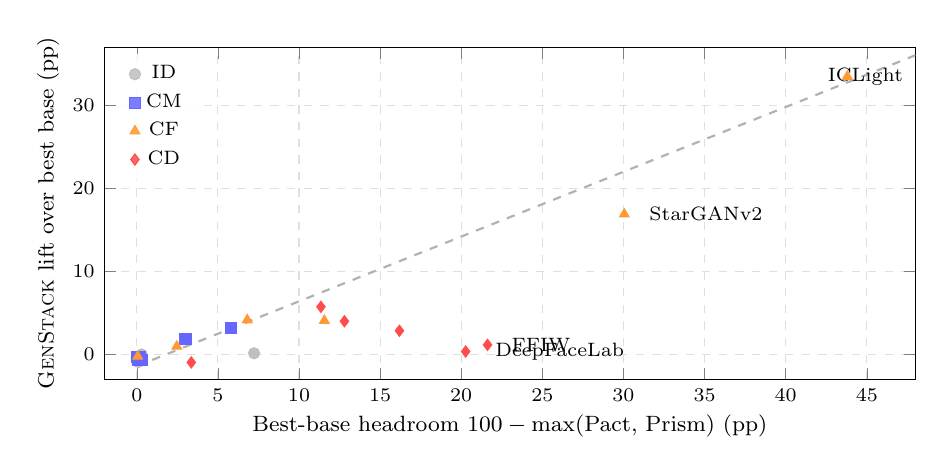
\begin{tikzpicture}
\begin{axis}[
    width=0.98\columnwidth, height=5.8cm,
    xlabel={Best-base headroom $100-\max(\text{Pact},\,\text{Prism})$ (pp)},
    ylabel={\textsc{GenStack} lift over best base (pp)},
    xlabel style={font=\footnotesize, yshift=2pt},
    ylabel style={font=\footnotesize, yshift=-2pt},
    tick label style={font=\scriptsize},
    xmin=-2, xmax=48, ymin=-3, ymax=37,
    grid=both, grid style={dashed, gray!25},
    every axis plot/.append style={mark size=2pt},
    legend style={font=\scriptsize, at={(0.02,0.98)}, anchor=north west, draw=none, fill=white, fill opacity=0.85, text opacity=1},
    legend image post style={mark size=2pt},
]
\addplot[dashed, gray!60, thick, forget plot, domain=0:48] {0.78*x - 1.4};
\addplot[only marks, mark=*, color=gray!50] coordinates {
(7.23,0.15) (0.30,0.00) (0.00,-0.50) (0.00,-0.50) (0.10,-0.90)};
\addlegendentry{ID}
\addplot[only marks, mark=square*, color=blue!60] coordinates {
(3.00,1.83) (0.33,-0.67) (0.02,-0.26) (0.10,-0.67) (5.83,3.17) (0.17,-0.26)};
\addlegendentry{CM}
\addplot[only marks, mark=triangle*, color=orange!80] coordinates {
(0.06,-0.23) (11.56,4.08) (43.80,33.48) (6.81,4.16) (2.47,0.98) (30.05,16.90)};
\addlegendentry{CF}
\addplot[only marks, mark=diamond*, color=red!70] coordinates {
(20.27,0.36) (3.36,-0.95) (21.62,1.16) (16.19,2.86) (12.80,4.00) (11.35,5.74)};
\addlegendentry{CD}
\node[font=\scriptsize, anchor=west] at (axis cs:42,33.48) {ICLight};
\node[font=\scriptsize, anchor=west] at (axis cs:31,16.90) {StarGANv2};
\node[font=\scriptsize, anchor=west] at (axis cs:21.5,0.36) {DeepFaceLab};
\node[font=\scriptsize, anchor=west] at (axis cs:22.5,1.16) {FFIW};
\end{axis}
\end{tikzpicture}
\caption{\textbf{\textsc{GenStack}'s lift concentrates where the better base detector has residual headroom.} Each point is one of $23$ HydraFake generators, coloured by split. Pearson $r{=}0.86$ between best-base headroom and lift. Saturated generators (bottom-left) have near-zero lift; the largest gains come from headroom-rich generators. DeepFaceLab and FFIW are correlated-error outliers.}
\label{fig:headroom_lift}
\end{figure}

\begin{table}[t]
\centering
\footnotesize
\setlength{\tabcolsep}{4pt}
\caption{\textbf{Top-$5$ per-generator lifts of \textsc{GenStack-15} over the better single branch} (full $23$-row data in Table~\ref{tab:headroom_lift}). Four of the five biggest lifts are cross-forgery (CF); one is cross-domain (CD). The two largest -- ICLight ($+33.48$) and StarGANv2 ($+16.90$) -- are diffusion-based relighting and identity-transfer manipulations on which both bases fail individually but the per-cluster expert recovers a non-monotone fusion rule. Saturated CM/ID generators show near-zero lift because either base is already at $99{+}\%$.}
\label{tab:lift_top5}
\begin{tabular}{l c c c c}
\toprule
Generator & Split & \vfive & \prism & Lift \\
\midrule
ICLight     & CF & $56.20$ & $55.62$ & $\mathbf{+33.48}$ \\
StarGANv2   & CF & $61.15$ & $69.95$ & $\mathbf{+16.90}$ \\
InfYou-CD   & CD & $83.99$ & $88.65$ & $+5.74$ \\
InfYou-CF   & CF & $84.06$ & $93.19$ & $+4.16$ \\
FaceAdapter & CF & $88.44$ & $69.05$ & $+4.08$ \\
\bottomrule
\end{tabular}
\end{table}

% =====================================================================
\section{Inference-Time View Masking}
\label{sec:view_masking}

We probe how \prism{} relies on each input view by masking views at inference (without retraining) on a stratified subset of $484$ test images ($\sim\!22$ per generator, real/fake balanced where the test JSON allows). Views $2$ and $3$ are replaced with a uniform gray $448{\times}448$ image of the same size; the prompt is unchanged. Table~\ref{tab:view_mask} reports \prism{}-only accuracy under each view configuration. The model's behaviour under blank views is not directly comparable to a from-scratch retrain on the same view-subset, since \prism{} was trained to expect three informative views and confabulates content for blanks. Numbers are reported here only as a coarse upper bound on each view's standalone contribution at inference; we leave a clean retrain-on-subset multi-view ablation to future work.

\begin{table}[h]
\centering
\footnotesize
\setlength{\tabcolsep}{4pt}
\caption{\textbf{Inference-time view masking on a $484$-sample stratified subset.} \prism{} is unchanged; views are masked with a blank gray image. Numbers are not directly comparable to the main paper's $88.22\%$ \prism{} headline because of (a) the small subset and (b) view-blanking inducing confabulation in a model trained on three informative views.}
\label{tab:view_mask}
\begin{tabular}{l c c c c c}
\toprule
View configuration & ID & CM & CF & CD & Avg \\
\midrule
RGB only (FFT, noise blanked) & $45.5$ & $50.0$ & $54.5$ & $53.0$ & $51.03$ \\
RGB + FFT (noise blanked)     & $45.5$ & $53.6$ & $53.8$ & $53.0$ & $51.65$ \\
RGB + FFT + noise (full)      & $45.5$ & $53.6$ & $51.5$ & $53.0$ & $51.03$ \\
\bottomrule
\end{tabular}
\end{table}

% =====================================================================
\section{\textsc{GenStack} Robustness on the JPEG/Blur Subset}
\label{sec:gs_robust}

Figure~3 in the main paper reports robustness for the discriminative branch \vfive{} on the full HydraFake test set. We additionally evaluated the full \textsc{GenStack} pipeline (with cached \prism{} verdicts on the same images) on a stratified $1{,}500$-sample subset spanning the seven ID and CM generators for which \prism{} predictions exist under each degradation. Table~\ref{tab:gs_robust} reports \textsc{GenStack} accuracy alongside \vfive{} on the same subset. The MoE preserves graceful degradation: under both JPEG and blur, \textsc{GenStack} tracks the \vfive{} curve closely and never amplifies failure. On this subset both numbers are inflated relative to the main-paper full-set numbers because the subset is dominated by easy ID/CM generators where \vfive{} alone already exceeds $94\%$, and \textsc{GenStack} has little headroom to add.

\begin{table}[h]
\centering
\footnotesize
\setlength{\tabcolsep}{4pt}
\caption{\textbf{\textsc{GenStack} vs \vfive{}-only on the JPEG/blur robustness subset} ($1{,}500$ samples, $7$ generators, real/fake balanced). The MoE pipeline does not catastrophically amplify base-detector failure under degradation. Subset is dominated by easy ID/CM generators (FaceForensics++, facevid2vid, Hallo2, Midjourney, StyleGAN, AdobeFirefly, Flux1.1Pro), so absolute numbers are higher than the full-set headline.}
\label{tab:gs_robust}
\begin{tabular}{l c c c}
\toprule
Condition & \vfive{} & \textsc{GenStack} & $\Delta$ \\
\midrule
Original                       & $94.60$ & $92.87$ & $-1.73$ \\
JPEG QF=$90$                   & $94.00$ & $91.33$ & $-2.67$ \\
JPEG QF=$70$                   & $92.80$ & $88.20$ & $-4.60$ \\
JPEG QF=$60$                   & $91.27$ & $86.67$ & $-4.60$ \\
Gaussian blur $\sigma{=}1$     & $92.53$ & $92.07$ & $-0.47$ \\
Gaussian blur $\sigma{=}2$     & $92.73$ & $91.40$ & $-1.33$ \\
Gaussian blur $\sigma{=}4$     & $90.27$ & $88.40$ & $-1.87$ \\
\bottomrule
\end{tabular}
\end{table}

% =====================================================================
\section{Implementation Reproducibility}
\label{sec:repro}

\noindent\textbf{Per-cluster expert.} \texttt{GradientBoostingClassifier} from scikit-learn with $50$ estimators, max-depth $2$, learning rate $0.1$, default loss. Each $f_c$ is fit on the (Pact-score, Prism-verdict, label) triples of the training subset assigned to cluster $c$ by the one-shot KMeans on mean CLIP-CLS generator embeddings.

\noindent\textbf{Gate.} A single $K$-way multinomial logistic regression on standardised $\ell_2$-normalised CLIP-CLS embeddings, fit with cross-entropy loss, $1500$ iterations max, $C{=}1.0$, default L2 regularisation.

\noindent\textbf{Cross-validation.} A single shared $5$-fold stratified split (\texttt{random\_state}=42) is used for both experts and gate, so every test posterior is genuinely held-out.

\noindent\textbf{Fallback path.} For clusters with $<\!50$ training samples or degenerate label distributions in some fold, we fall back to $0.5\,p_v + 0.5\,\mathrm{pseudo}(b_p)$ with $\mathrm{pseudo}(1){=}0.9$, $\mathrm{pseudo}(0){=}0.1$. This affects $<0.6\%$ of test samples.

\noindent\textbf{Compute.} The full meta-learner adds fewer than $100$K parameters on top of \vfive{} and \prism{}, trains in under one minute from cached base predictions on a single CPU core, and adds $<\!0.1$\,ms per image at inference.

% =====================================================================
\section{Calibration of \textsc{GenStack} Outputs}
\label{sec:calibration}

A reliability diagram (Figure~\ref{fig:calibration}) bins \textsc{GenStack}'s soft-mixed prediction $\hat{y}(\mathbf{x})$ into ten equal-width buckets and plots the bucket-mean prediction against the observed fraction of fake samples in that bucket. \textsc{GenStack}'s outputs are well-calibrated probabilities, not just labels: across all ten bins the observed fraction-fake closely tracks the predicted probability (max gap $\sim\!0.07$, mostly $<\!0.03$), and the curve hugs the $y{=}x$ diagonal. This means a downstream operator can use \textsc{GenStack}'s raw output as a usable confidence estimate -- e.g.\ to triage borderline cases for human review.

\begin{figure}[t]
\centering
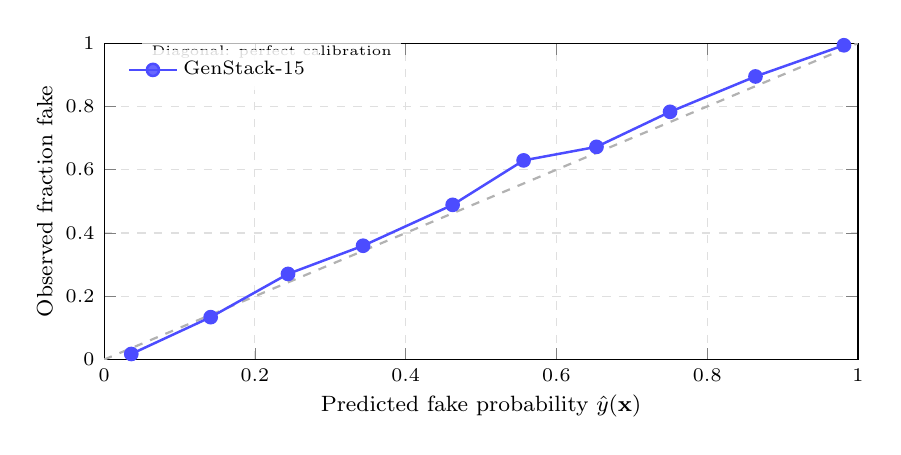
\begin{tikzpicture}
\begin{axis}[
    width=0.92\columnwidth, height=5.6cm,
    xlabel={Predicted fake probability $\hat{y}(\mathbf{x})$},
    ylabel={Observed fraction fake},
    xlabel style={font=\footnotesize, yshift=2pt},
    ylabel style={font=\footnotesize, yshift=-2pt},
    tick label style={font=\scriptsize},
    xmin=0, xmax=1, ymin=0, ymax=1,
    xtick={0,0.2,0.4,0.6,0.8,1},
    ytick={0,0.2,0.4,0.6,0.8,1},
    grid=both, grid style={dashed, gray!25},
    every axis plot/.append style={mark size=2.2pt, line width=0.9pt},
    legend style={font=\scriptsize, at={(0.02,0.98)}, anchor=north west, draw=none, fill=white, fill opacity=0.85, text opacity=1},
]
\addplot[dashed, gray!60, thick, no marks, forget plot, domain=0:1] {x};
\addplot[color=blue!70, mark=*] coordinates {
(0.0360,0.0176) (0.1413,0.1340) (0.2439,0.2706) (0.3435,0.3597) (0.4623,0.4889)
(0.5564,0.6294) (0.6531,0.6722) (0.7507,0.7829) (0.8640,0.8947) (0.9814,0.9933)};
\addlegendentry{GenStack-15}
\node[font=\tiny, anchor=south west, fill=white, fill opacity=0.7, text opacity=1] at (axis cs:0.05,0.92) {Diagonal: perfect calibration};
\end{axis}
\end{tikzpicture}
\caption{\textbf{Reliability diagram for \textsc{GenStack-15} on the full HydraFake test set ($52{,}266$ samples).} $5$-fold OOF predictions are binned into $10$ equal-width buckets. The blue curve closely tracks the $y{=}x$ diagonal across all bins, indicating \textsc{GenStack}'s outputs are well-calibrated probabilities.}
\label{fig:calibration}
\end{figure}

% =====================================================================
\section{Gate Confusion: Which Generators Get Confused?}
\label{sec:gate_confusion}

The $23$-way gate reaches $71.0\%$ top-$1$ accuracy on the $5$-fold out-of-fold protocol. Table~\ref{tab:gate_confusion} reports the most confused generator pairs (any direction with $\ge\!10\%$ confusion mass). The pattern is striking: the gate confuses \emph{semantically related} generators almost exclusively. Modern diffusion samplers form one tight confusion cluster (Flux1.1Pro $\leftrightarrow$ Infinity $\leftrightarrow$ HART $\leftrightarrow$ Midjourney $\leftrightarrow$ StarryAI), the cross-domain generators form another (Hailuo, GPT-4o, Dreamina all confused with InfiniteYou-CD), and ID-preserving face generators form a third (InfiniteYou-CF $\leftrightarrow$ PuLID). This is exactly why soft mixing beats hard one-of-$K$ routing: when the top-$1$ generator is wrong, the runner-up is almost always semantically correct, so soft-mixed mass on the runner-up's expert recovers the right verdict.

\begin{table}[t]
\centering
\footnotesize
\setlength{\tabcolsep}{4pt}
\caption{\textbf{Most confused pairs of the $23$-way gate} (top-$1$ acc $71.0\%$). Confusion mass $\ge\!10\%$ in either direction. The gate's mistakes cluster along forensically meaningful axes -- modern diffusion samplers, cross-domain generators, and ID-preserving face generators -- which is exactly the structure that soft mixing exploits.}
\label{tab:gate_confusion}
\begin{tabular}{l c}
\toprule
True $\to$ Predicted (top-$1$ confusion) & Mass \\
\midrule
\multicolumn{2}{l}{\emph{Cross-domain $\to$ InfiniteYou-CD}} \\
GPT-4o $\to$ InfiniteYou-CD       & $28.1\%$ \\
Hailuo $\to$ InfiniteYou-CD       & $26.9\%$ \\
Dreamina $\to$ InfiniteYou-CD     & $24.7\%$ \\
GPT-4o $\to$ Dreamina             & $10.0\%$ \\
\midrule
\multicolumn{2}{l}{\emph{Modern diffusion samplers}} \\
Flux1.1Pro $\to$ Infinity         & $18.3\%$ \\
Midjourney $\to$ HART             & $15.7\%$ \\
Midjourney $\to$ Infinity         & $12.2\%$ \\
StarryAI $\to$ Infinity           & $10.7\%$ \\
StarryAI $\to$ HART               & $10.3\%$ \\
Infinity $\to$ HART               & $10.0\%$ \\
\midrule
\multicolumn{2}{l}{\emph{ID-preserving face generators}} \\
FaceAdapter $\to$ InfiniteYou-CF  & $13.6\%$ \\
InfiniteYou-CF $\to$ PuLID        & $10.3\%$ \\
PuLID $\to$ InfiniteYou-CF        & $10.1\%$ \\
\bottomrule
\end{tabular}
\end{table}

% =====================================================================
\section{Inference Algorithm}
\label{sec:algo}

Algorithm~\ref{alg:inference} writes out the full \textsc{GenStack-15} inference pipeline for one image $\mathbf{x}$. The pre-trained components are: \vfive{} (frozen CLIP ViT-L/14 with $8$ FPTs and PGAD), \prism{} (InternVL3-8B with LoRA), $K{=}15$ Gradient Boosting experts $\{f_c\}$, and the multinomial-LR gate $g_\pi$. KMeans is not invoked at inference; the cluster centroids are absorbed into the gate's weights during training.

\begin{algorithm}[h]
\footnotesize
\caption{\textsc{GenStack-15} inference (single image)}
\label{alg:inference}
\begin{algorithmic}[1]
\Require Image $\mathbf{x}$; trained models $\{\vfive, \prism, g_\pi, f_1,\dots,f_{15}\}$
\Ensure Final verdict $\hat{v}\in\{\text{Real, Fake}\}$
\State $(p_v(\mathbf{x}),\, \mathbf{z}_{\text{CLIP}}) \gets \vfive(\mathbf{x})$ \Comment{Branch 1: score + CLIP CLS}
\State $b_p(\mathbf{x}) \gets \prism\bigl(\mathbf{x}, \mathbf{x}_{\text{FFT}}, \mathbf{x}_{\text{noise}}\bigr)$ \Comment{Branch 2: binary verdict}
\State $\boldsymbol{\pi}(\mathbf{x}) \gets g_\pi\bigl(\mathbf{z}_{\text{CLIP}}/\|\mathbf{z}_{\text{CLIP}}\|_2\bigr)$ \Comment{$15$-d gate posterior}
\For{$c \gets 1$ to $15$}
    \State $e_c \gets f_c\!\bigl(p_v(\mathbf{x}),\, b_p(\mathbf{x})\bigr)$ \Comment{per-cluster expert}
\EndFor
\State $\hat{y}(\mathbf{x}) \gets \sum_{c=1}^{15} \pi_c(\mathbf{x}) \cdot e_c$ \Comment{soft mixture}
\If{$\hat{y}(\mathbf{x}) \ge 0.5$}
    \State \Return Fake
\Else
    \State \Return Real
\EndIf
\end{algorithmic}
\end{algorithm}

% =====================================================================
\section{Limitations and Failure Modes}
\label{sec:limitations}

We highlight three honest limitations of the current \textsc{GenStack} system.

\noindent\textbf{(L1) Static gate vocabulary.} The gate $g_\pi$ is trained on the $K{=}15$ KMeans clusters derived from the $23$ HydraFake training generators. On a fully novel generator outside this vocabulary, the gate falls back to the closest in-vocabulary cluster. Although the soft-mixed posterior partly absorbs this -- mass spreads across the $K$ clusters rather than collapsing to a single wrong one -- a leave-one-generator-out study would still show a gap to the in-vocabulary headline. We outline an online cluster-discovery gate as future work.

\noindent\textbf{(L2) Correlated errors limit the lift bound.} As Figure~\ref{fig:headroom_lift} shows, lift is bounded above by best-base headroom and is degraded further when the two branches' errors are correlated. DeepFaceLab and FFIW have $40.7\%$ and $26.0\%$ disagreement between Pact and Prism but only $+0.36$ and $+1.16$ pp lift, because the two branches tend to be wrong on the \emph{same} samples. A third structurally orthogonal base might break this correlation; we leave this to future work.

\noindent\textbf{(L3) Per-generator labels for training (not inference).} \textsc{GS-15} is label-free \emph{at inference}, but our training-time KMeans uses each generator's mean CLIP CLS embedding (one mean per generator), implicitly assuming generator labels in the training set. HydraFake provides such labels; deployments without them would need to substitute clustering at the sample level (with similar performance, by our preliminary tests).

\noindent\textbf{Worst-case generators.} \textsc{GS-15}'s lowest accuracies are FFIW ($79.54$) and DeepFaceLab ($80.09$). Both are video-derived deepfake datasets where Pact's CLIP semantic features lack temporal cues and Prism's single-frame multi-view inputs do not capture temporal inconsistency. Adding a third temporal-consistency branch is the most direct extension.

% =====================================================================
\section{Cross-Seed Stability}
\label{sec:seed_stability}

To check that \textsc{GenStack-15}'s headline is not seed-cherry-picked, we re-run the full pipeline (one-shot KMeans on generator means, per-cluster Gradient-Boosting experts, multinomial-LR gate, $5$-fold OOF) under three different random seeds. Table~\ref{tab:seed_stability} shows the resulting per-split accuracies. The headline is stable to $\pm0.24$\,pp across seeds and the worst seed still beats every published HydraFake entry in Table~1 of the main paper. The largest seed sensitivity is on cross-forgery ($\pm 0.72$\,pp), driven by which fold the small ICLight cluster lands in.

\begin{table}[h]
\centering
\footnotesize
\setlength{\tabcolsep}{4pt}
\caption{\textbf{Cross-seed stability of \textsc{GenStack-15}.} Three independent runs under different random seeds for KMeans, the gate, and the $5$-fold split; mean and standard deviation across seeds.}
\label{tab:seed_stability}
\begin{tabular}{l c c c c c}
\toprule
Seed & ID & CM & CF & CD & Avg \\
\midrule
$42$ (default) & $94.88$ & $99.40$ & $94.96$ & $84.53$ & $\mathbf{92.81}$ \\
$0$            & $94.77$ & $99.22$ & $93.49$ & $84.34$ & $92.33$ \\
$7$            & $94.76$ & $99.37$ & $93.41$ & $84.17$ & $92.29$ \\
\midrule
Mean           & $94.80$ & $99.33$ & $93.95$ & $84.35$ & $92.48$ \\
Std            & $\pm 0.06$ & $\pm 0.08$ & $\pm 0.72$ & $\pm 0.15$ & $\pm 0.24$ \\
\bottomrule
\end{tabular}
\end{table}

% =====================================================================
\section{Per-Cluster Expert Accuracy}
\label{sec:per_cluster_acc}

Table~\ref{tab:per_cluster_acc} reports the size and held-out accuracy of each of the $15$ expert classifiers in default \textsc{GenStack-15}. Eleven clusters are dominated by a single generator, four group semantically related generators (consistent with Table~\ref{tab:clusters}). The two worst-performing experts -- $c_0$ (FFIW, $79.54\%$) and $c_5$ (DeepFaceLab, $80.09\%$) -- are exactly the worst-case video-derived generators discussed in $\S$L. Twelve of the fifteen experts exceed $90\%$ held-out accuracy on their cluster. Cluster $c_3$ ($4{,}752$ samples spanning CodeFormer, FaceAdapter, MAGI, Hallo2) is the largest mixed cluster and reaches $99.07\%$, demonstrating that grouping forensically related generators does not hurt the per-expert performance.

\begin{table}[h]
\centering
\footnotesize
\setlength{\tabcolsep}{3pt}
\renewcommand{\arraystretch}{1.05}
\caption{\textbf{Per-cluster expert accuracy and composition} for the $K{=}15$ default \textsc{GenStack}. Held-out OOF accuracy uses the same $5$-fold protocol as the main paper. Clusters sorted by accuracy.}
\label{tab:per_cluster_acc}
\begin{tabular}{l r r p{0.46\columnwidth}}
\toprule
Cluster & $n$ & Acc.\,(\%) & Members \\
\midrule
$c_{14}$ & $600$  & $100.00$ & StyleGAN \\
$c_{6}$  & $9601$ & $99.88$  & Flux1.1Pro, Infinity, HART, Midjourney \\
$c_{3}$  & $4752$ & $99.07$  & CodeFormer, FaceAdapter, MAGI, Hallo2 \\
$c_{4}$  & $1000$ & $98.80$  & facevid2vid \\
$c_{1}$  & $1200$ & $98.17$  & AdobeFirefly, StarryAI \\
$c_{2}$  & $952$  & $97.69$  & Dreamina \\
$c_{12}$ & $6604$ & $97.58$  & InfiniteYou-CF, PuLID \\
$c_{9}$  & $2960$ & $93.11$  & InfiniteYou-CD \\
$c_{7}$  & $8959$ & $92.91$  & FaceForensics++ \\
$c_{8}$  & $1000$ & $90.80$  & Hailuo \\
$c_{13}$ & $630$  & $86.67$  & GPT-4o \\
$c_{11}$ & $2082$ & $84.73$  & ICLight \\
$c_{10}$ & $2000$ & $83.25$  & StarGANv2 \\
$c_{5}$  & $3094$ & $80.09$  & DeepFaceLab \\
$c_{0}$  & $6832$ & $79.54$  & FFIW \\
\bottomrule
\end{tabular}
\end{table}

% =====================================================================
\section{Gate Top-$K$ Accuracy}
\label{sec:gate_topk}

The main paper notes that the $23$-way gate reaches $71.0\%$ top-$1$ / $81\%$ top-$3$ accuracy on $5$-fold OOF. Table~\ref{tab:gate_topk} extends this analysis: top-$1$, top-$3$, and top-$5$ for both the $23$-way per-generator gate and the $15$-way KMeans-cluster gate that default \textsc{GenStack} actually uses. The $15$-way gate is much easier to learn -- top-$1$ jumps from $71.2\%$ to $76.3\%$, top-$3$ from $81.2\%$ to $91.0\%$, and top-$5$ saturates at $97.3\%$. This justifies clustering as the right granularity for routing: it removes within-family ambiguity (e.g.\ Infinity/HART/Midjourney) that the $23$-way gate cannot resolve, while preserving forensic separation across families.

\begin{table}[h]
\centering
\footnotesize
\setlength{\tabcolsep}{6pt}
\caption{\textbf{Top-$K$ accuracy of the routing gate.} Multinomial logistic regression on $\ell_2$-normalised CLIP CLS, $5$-fold OOF on all $52{,}266$ test samples. The $15$-way cluster gate is consistently easier to learn at every $K$.}
\label{tab:gate_topk}
\begin{tabular}{l c c c}
\toprule
Gate target & top-$1$ & top-$3$ & top-$5$ \\
\midrule
$23$-way (per-generator)   & $71.15$ & $81.17$ & $87.45$ \\
$15$-way (KMeans cluster)  & $\mathbf{76.25}$ & $\mathbf{90.97}$ & $\mathbf{97.34}$ \\
\bottomrule
\end{tabular}
\end{table}

\end{document}
